\documentclass[paper.tex]{subfiles}

\usepackage{tikz}
\usepackage{amsmath}
\usepackage{graphicx}
\usepackage{tabularx}
\usepackage{multicol}
\usepackage{algpseudocode}
\usepackage{algorithm}

% Add vertical spacing to tables
\renewcommand{\arraystretch}{1.4}

% Begin Document
\begin{document}

\section{Introduction}

In this paper, we explore the Minimum Dominating Set of a Graph and how to find it.
The Minimum Domianting Set of a Graph is the Set of all nodes such that every node or one of its neighbors is in the set.

This paper is divided into the following sections. 
Section 2 contains background information on the Minimum Dominating Set.
Section 3 contains the algorithm used to solve for the Minimum Dominating Set.
Section 4 contains experimental data when running the algorithm.
Section 5 concludes the paper.

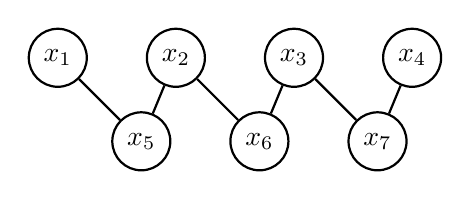
\begin{tikzpicture}[node distance={15mm}, thick, main/.style = {draw, circle}] 
    \node[main] (1) {$x_1$};  
    \node[main] (2) [right of = 1] {$x_2$};  
    \node[main] (3) [right of = 2] {$x_3$};  
    \node[main] (4) [right of = 3] {$x_4$};
    \node[main] (5) [below right of = 1] {$x_5$};
    \node[main] (6) [below right of = 2] {$x_6$};
    \node[main] (7) [below right of = 3] {$x_7$};  
    \draw (1) -- (5);
    \draw (2) -- (5);
    \draw (2) -- (6);
    \draw (3) -- (6);
    \draw (3) -- (7);
    \draw (4) -- (7);  
\end{tikzpicture}


\end{document}